\subsection{Bovine \textit{IFIT} Responses to Activators of Innate Immune Response} \label{subsec:Bovine IFIT Responses to Activators of Innate Immune Response}
The Madin-Darby bovine kidney (MDBK) cell line, derived from bovine renal epithelium in 1958 (\cite{Madin1958EstablishedOrigin}), is a well-established model system used in bovine virology studies. We assayed the cells for the induction potential of bovine \textit{IFITs}, alongside bovine \textit{Mx1} using bovine interferon alpha and LPS (bovine interferon-gamma was not available commercially). Bovine \textit{Mx1} was included in the analyses as it is a ISG, widely reported in immunology and virology studies (ADD SOME REFERENCES HERE FOR CRYING OUT LOUD), and because we saw minimal bovine \textit{IFIT} responses throughout the study and wanted to ensure the cell lines used had the internal pathways for ISG induction correctly functioning. Figure \ref{fig:MDBK responses to bIFNa} shows the \textit{bIFIT} and \textit{bMx1} responses to the stimulation with bIFN\(\alpha\) at a concentration of 5 ng/mL (equivalent to 1,000 UI/mL of hIFN\(\alpha\)) for either 3 or 6 hours. Interestingly, we see a similar effect in induction amplitude but an opposing effect in time of stimulation to amplitude compared to hIFN\(\alpha\) induction in BEAS-2B cells (Figure \ref{fig:BEAS-2B responses to hIFNa}). DESCRIBE THE DATA ITSELF ....


all ifits:
    sig at 3
        1 highest, 2 3 the same, 5 lowest (like a549)
    higher 3 than 6
    1 sig at 6
    bmx1 sig at both
        3 double 1
        6 even higher (4x)
        shows that ifn stim worked and ifits are fast acting fast degrading
        also shows mdbk ifits are competent and ifn cascades work

normal unequal - bi1 bi2 bmx1

normal equal - bi3 bi5

mdbk bifna stim

bMx1 was induced by all bIFN alpha at different concentrations and timepoints, but at 5 ng/mL for 24h. This means that either that treatment failed or 24h post adding the bIFN treatment is too late to capture the ISG induction. All targets are induced by bIFN alpha treatment at 5 ng/mL for 3 hours. bIFIT1 also responds to low concentration (0.5 ng/mL) for 6h treatment, but not the other IFITs. No other concentration/time combination induced bIFITs. 

This all suggests that MDBK are responsive to bIFN alpha and capable of bIFIT induction, but the responses are week, especially compared to human cells.

I have a hypothesis that in bovine cells the IFITs are basally expressed to higher levels  (that would explain why we can detect them by IF in mock and infected cell although the qPCR data suggest there is no induction).

\begin{figure}
    \centering
    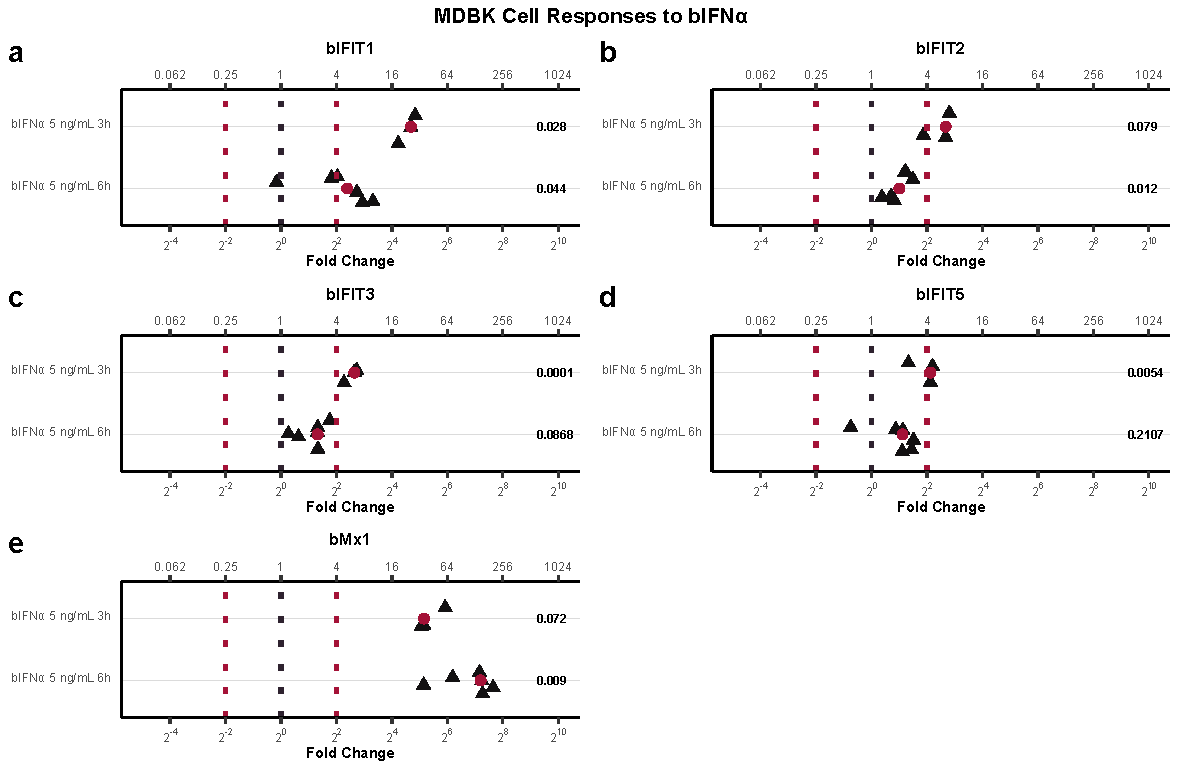
\includegraphics[width=1\linewidth]{07. Chapter 2/Figs/02. Induction/01. mdbk_treat_bifna.pdf}
    \caption[\textit{bIFIT} Gene Expression in MDBK Cells in Response to bIFN\(\alpha\) Stimulation.]{\textbf{\textit{bIFIT} Gene Expression in MDBK Cells in Response to bIFN\(\alpha\) Stimulation.} (a) \textit{bIFIT1}, (b) \textit{bIFIT2}, (c) \textit{bIFIT3}, (d) \textit{bIFIT5}, and (e) \textit{bMx1} gene expression levels were assessed using quantitative real-time PCR (qPCR) in MDBK cells following stimulation with bovine interferon alpha (IFN\(\alpha\)) at a concentration of 5 ng/mL for a treatment duration of either 3 or 6 hours. Relative expression values are normalized to standardized mock-treated samples. Median values are represented by red circles. The black dotted line represents mock expression levels, while the red dotted lines indicate biologically significant induction thresholds. Numeric values indicate the p-values compared to mock-treated samples.}
    \label{fig:MDBK responses to bIFNa}
\end{figure}

mdbk lps

Neither bMx1 nor bIFITs are induced by LPS in the concentration range tested. 

nothing responding to lps
0.5 2.5 1, 2.5 2, 2.5 3 - inhibition by Half
    while no response in bmx1 and 5
    not biologically significant probs

normal unequal - bi1 bi2 

normal equal - bi3 bi5 bmx1


\begin{figure}
    \centering
    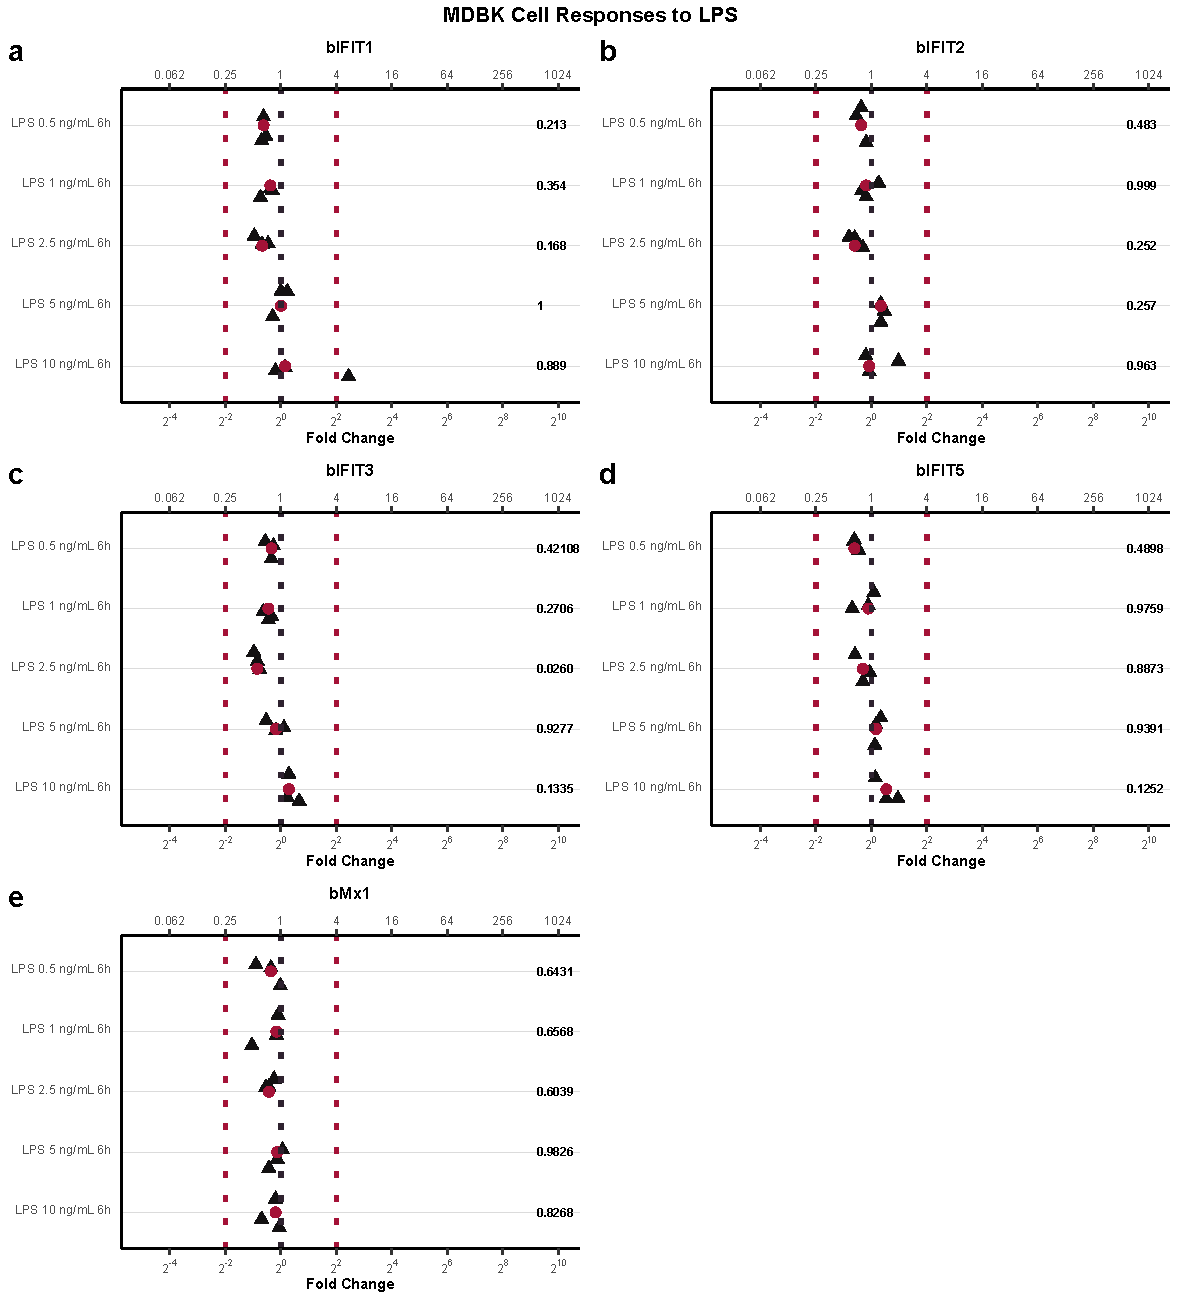
\includegraphics[width=1\linewidth]{07. Chapter 2/Figs/02. Induction/02. mdbk_treat_lps.pdf}
    \caption[\textit{bIFIT} Gene Expression in MDBK Cells in Response to LPS Stimulation.]{\textbf{\textit{bIFIT} Gene Expression in MDBK Cells in Response to LPS Stimulation.} (a) \textit{bIFIT1}, (b) \textit{bIFIT2}, (c) \textit{bIFIT3}, (d) \textit{bIFIT5}, and (e) \textit{bMx1} gene expression levels were assessed using quantitative real-time PCR (qPCR) in MDBK cells following stimulation with bacterial LPS at a concentration of 0.5, 1, 2.5, 5, and 10 ng/mL for a treatment duration of 6 hours. Relative expression values are normalized to standardized mock-treated samples. Median values are represented by red circles. The black dotted line represents mock expression levels, while the red dotted lines indicate biologically significant induction thresholds. Numeric values indicate the p-values compared to mock-treated samples.}
    \label{fig:MDBK responses to LPS}
\end{figure}

bt intro

bt bifna

% bt paper
(\cite{McClurkin1974ComparisonVirus})

Validation in more physiologically relevant cell line. All genes but bIFIT2 respond to bIFN alpha 5 ng/mL for 3h; treatment for 24h cause no change in any of the genes; treatment for 6h downregulates IFITs but not bMx1. This shows that BT cells are responsive to IFN and have the capability to express bIFITs and bMx1.

2 not responsive
everything else sig induction at 3 and minimal induction for bmx1 and 5 at 24
shows bt being ifit competent, ifn cascades work, fast action that doesnt last a day


normal unequal - bi1 bi3 bi5 bmx1

normal euqal - bi2 


\begin{figure}
    \centering
    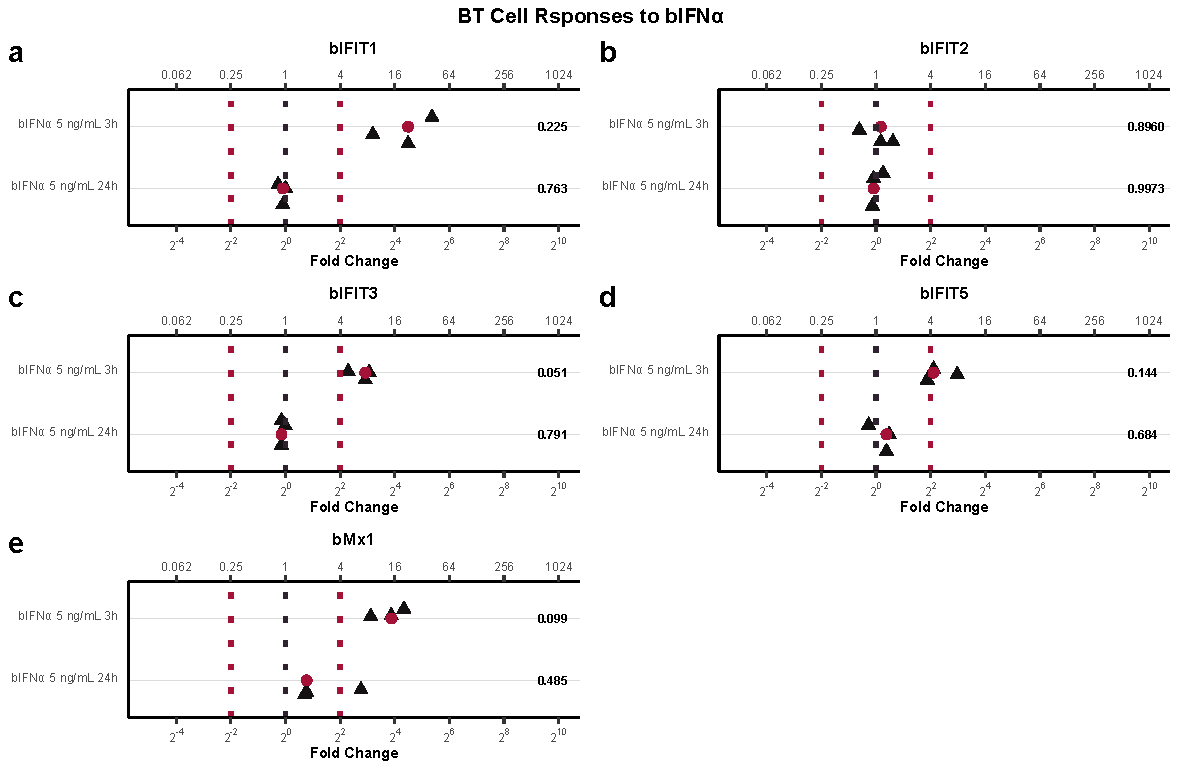
\includegraphics[width=1\linewidth]{07. Chapter 2/Figs/02. Induction/08. bt_bifna.pdf}
    \caption[\textit{bIFIT} Gene Expression in BT Cells in Response to bIFN\(\alpha\) Stimulation.]{\textbf{\textit{bIFIT} Gene Expression in BT Cells in Response to bIFN\(\alpha\) Stimulation.} (a) \textit{bIFIT1}, (b) \textit{bIFIT2}, (c) \textit{bIFIT3}, (d) \textit{bIFIT5}, and (e) \textit{bMx1} gene expression levels were assessed using quantitative real-time PCR (qPCR) in BT cells following stimulation with bovine interferon alpha (IFN\(\alpha\)) at a concentration of 5 ng/mL for a treatment duration of either 3 or 24 hours. Relative expression values are normalized to standardized mock-treated samples. Median values are represented by red circles. The black dotted line represents mock expression levels, while the red dotted lines indicate biologically significant induction thresholds. Numeric values indicate the p-values compared to mock-treated samples.}
    \label{fig:BT responses to bifna}
\end{figure}

\subsection{Bovine \textit{IFITs} Responses to bRSV} \label{subsec:Bovine IFITs Responses to bRSV}

intro about infections - methods and so


\begin{figure}
    \centering
    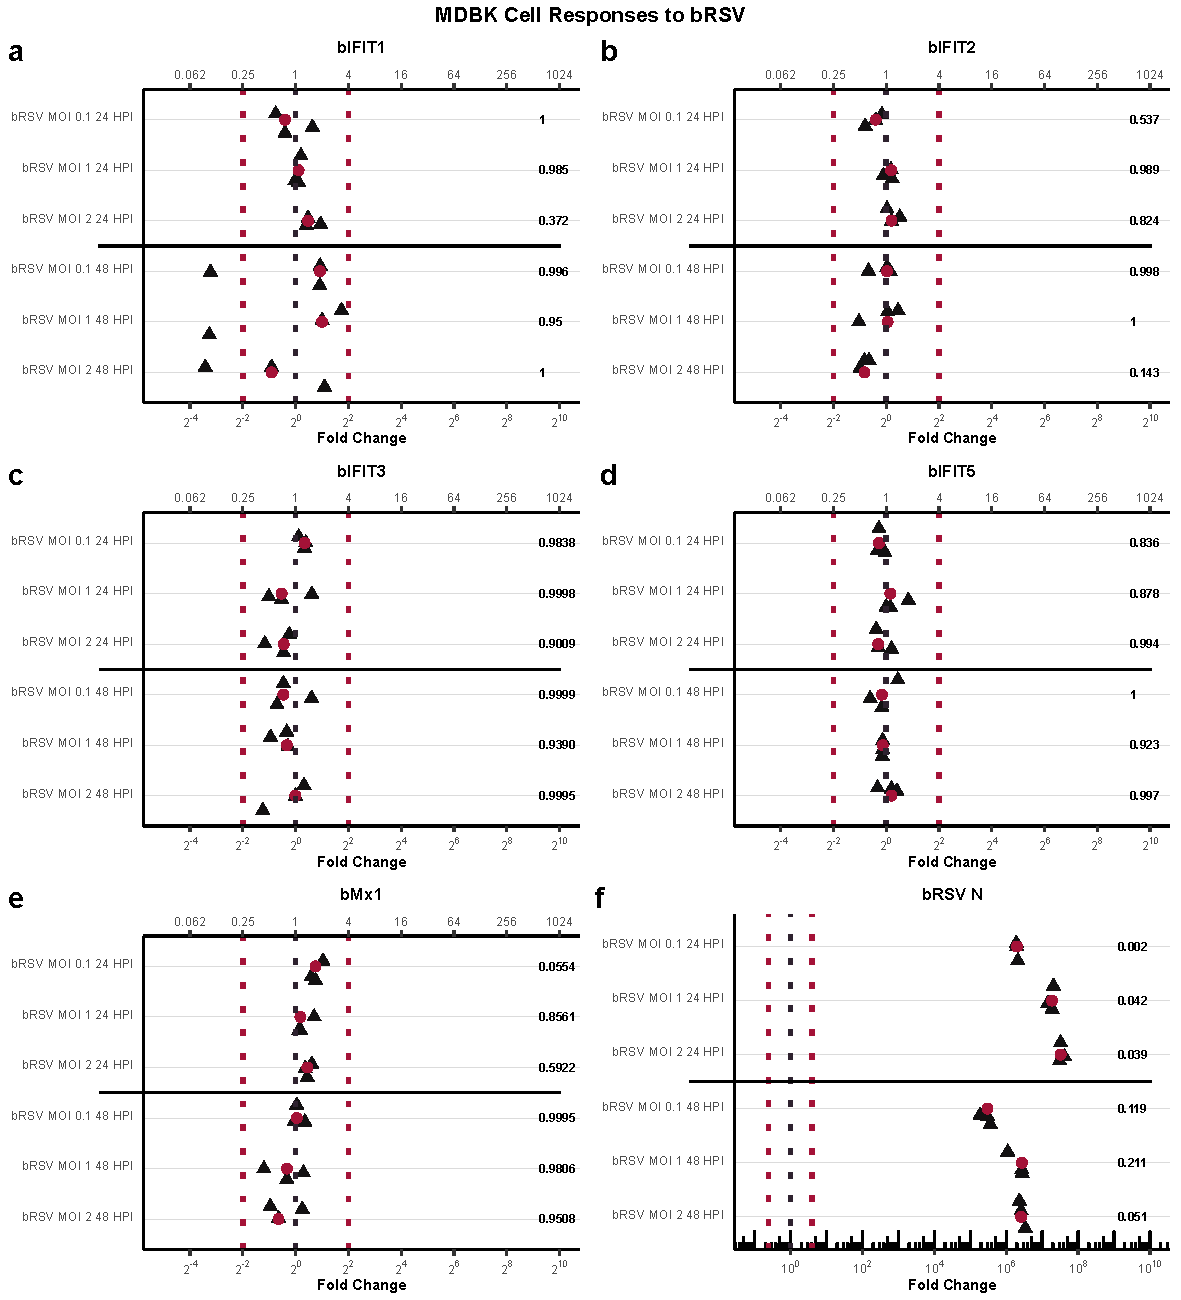
\includegraphics[width=1\linewidth]{07. Chapter 2/Figs/02. Induction/03. mdbk_brsv_timepoints.pdf}
    \caption[MDBK \textit{bIFIT} Response to bRSV Infection as a Function of Time and MOI.]{\textbf{MDBK \textit{bIFIT} Response to bRSV Infection as a Function of Time and MOI.} (a) \textit{bIFIT1}, (b) \textit{bIFIT2}, (c) \textit{bIFIT3}, (d) \textit{bIFIT5}, (e) \textit{bMx1} and (f) \textit{bRSV N} gene expression levels were assessed using quantitative real-time PCR (qPCR) in MDBK cell line following infection with bovine RSV at MOI of either 0.1, 1, or 2 for either 24 or 48 hours post-infection. Relative expression values are normalized to standardized mock-treated samples. Median values are represented by red circles. The black dotted line represents mock expression levels, while the red dotted lines indicate biologically significant induction thresholds. Numeric values indicate the p-values compared to mock-treated samples.}
    \label{fig:MDBK responses to bRSV timepoints}
\end{figure}

timepoints data

Low, mid, and high MOI (0.1, 1, 2) and two different time points (24 and 48 HPI) do not seem to influence the levels of any genes

no biologicaly sig response
very strong viral replication
1 48 0.1 1 half increase; 2 half decrease
2 48 2 half decrease
3 and 5 nothing
mx1 24 0.1 half increase; 48 2 half decrease
viruses replicating well but not stimulating; 48 should be quite high titre based on growth curves and still nothing

normal unequal - bi1 bi2  bi5 brsvn

normal euqal - bi3 bmx1

\begin{figure}
    \centering
    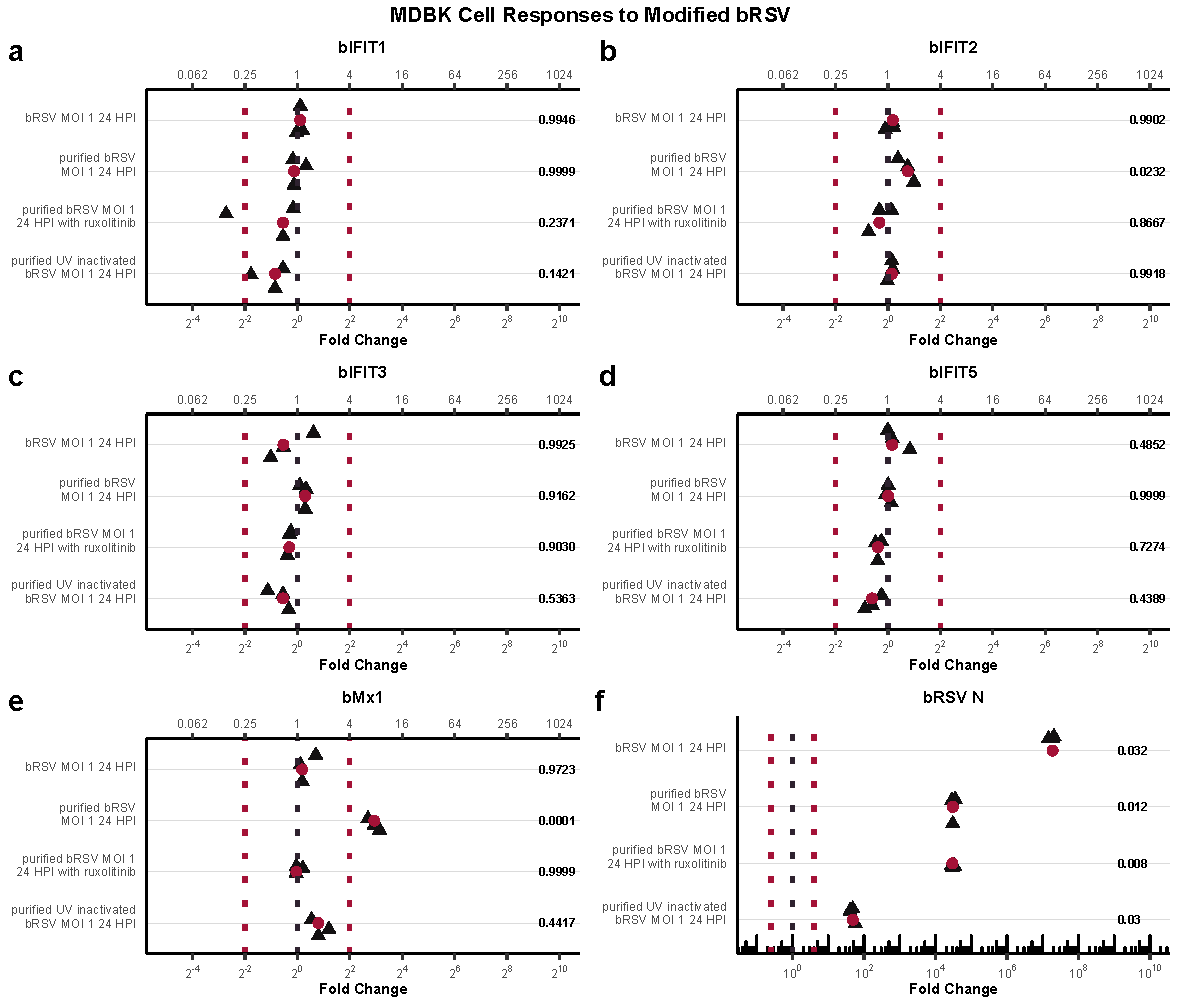
\includegraphics[width=1\linewidth]{07. Chapter 2/Figs/02. Induction/04. mdbk_brsv_uv_roxo.pdf}
    \caption[Impact of Ultra-Purification, UV-Inactivation, and INFR Inhibition on \textit{bIFIT} Induction in MDBK Cells Following bRSV Infection.]{\textbf{Impact of Ultra-Purification, UV-Inactivation, and INFR Inhibition on \textit{bIFIT} Induction in MDBK Cells Following bRSV Infection.} (a) \textit{bIFIT1}, (b) \textit{bIFIT2}, (c) \textit{bIFIT3}, (d) \textit{bIFIT5}, (e) \textit{bMx1}, and (f) \textit{bRSV N} gene expression levels were assessed using quantitative real-time PCR (qPCR) in MDBK cell line following infection with ultra-purified bRSV at MOI 1 for 24 hours. The cells were subjected to three different conditions: virus infection alone (top row), virus infection in the presence of 5 nM of ruxolitinib (interferon receptor inhibitor) throughout the infection (middle row), or UV-inactivated bRSV infection (bottom row). Relative expression values are normalized to standardized mock-treated samples. Median values are represented by red circles. The black dotted line represents mock expression levels, while the red dotted lines indicate biologically significant induction thresholds. Numeric values indicate the p-values compared to mock-treated samples.}
    \label{fig:The effect of ultra-purification, UV-inactivation and INFR inhibition on hIFIT induction following hRSV infection in MDBK}
\end{figure}


mdbk uv roxo puri

UV inactivated bRSV causes no change for bMx1 and bIFIT2 and seems to downregulate bIFIT1,3,5.

other than for bMx1 for wt ultracentrifugation purified bRSV 24 HPI MOI 1. I have one experiment where bRSV MOI 1 24 HPI downregulates all genes tested but it might be a technical error. 




normal unequal - bmx1 brsvn

normal euqal - bi1 bi2 bi3 bi5


\begin{figure}
    \centering
    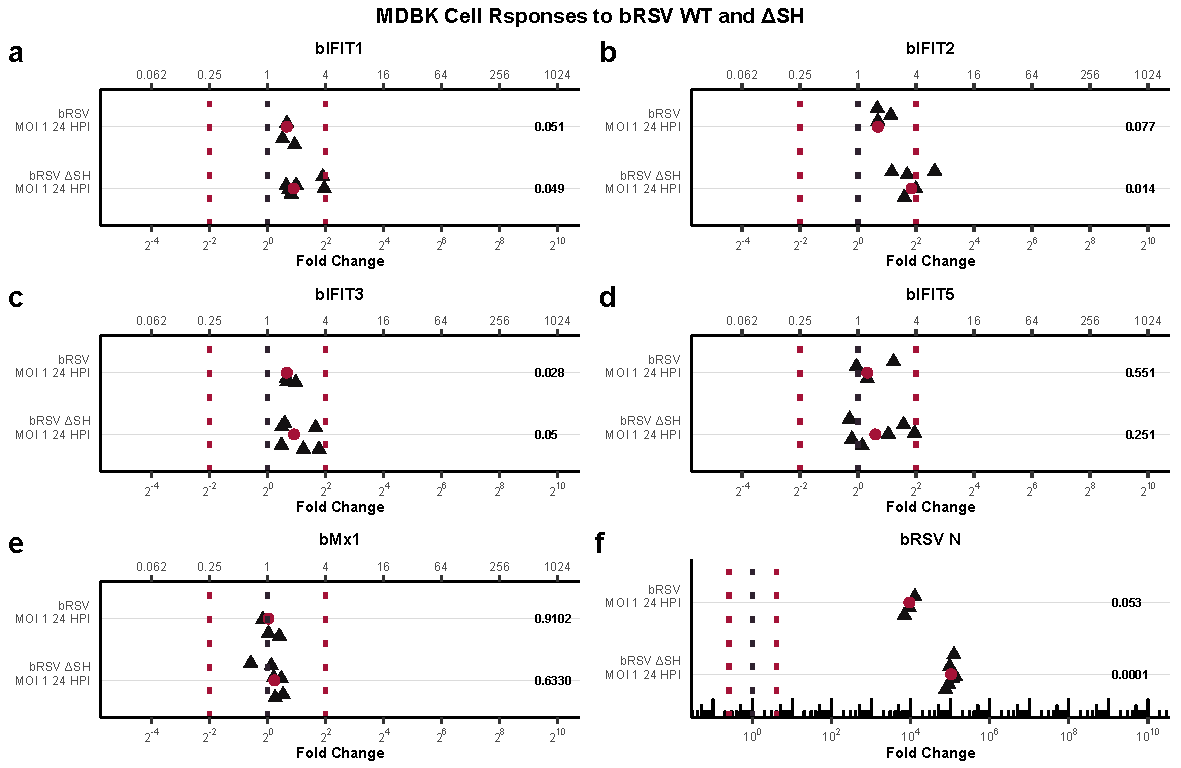
\includegraphics[width=1\linewidth]{07. Chapter 2/Figs/02. Induction/05. mdbk_brsv_moi1_dsh.pdf}
    \caption[MDBK \textit{bIFIT} Response to WT and \(\Delta\)SH bRSV Infection.]{\textbf{MDBK \textit{bIFIT} Response to WT and \(\Delta\)SH bRSV Infection.} (a) \textit{bIFIT1}, (b) \textit{bIFIT2}, (c) \textit{bIFIT3}, (d) \textit{bIFIT5}, (e) \textit{bMx1}, and (f) \textit{bRSV N} gene expression levels were assessed using quantitative real-time PCR (qPCR) in MDBK cell line following infection with WT or \(\Delta\)SH bRSV at MOI 1 for 24 hours post-infection. Relative expression values are normalized to standardized mock-treated samples. Median values are represented by red circles. The black dotted line represents mock expression levels, while the red dotted lines indicate biologically significant induction thresholds. Numeric values indicate the p-values compared to mock-treated samples.}
    \label{fig:MDBK responses to dSH}
\end{figure}



mdbk dsh

wt bRSV along with MOI 1 dSH do not up or downregulate any genes tested in a biologically significant way.

normal unequal - bi1 bi2 bi3 bi5 brsvn

normal euqal - bmx1


\begin{figure}
    \centering
    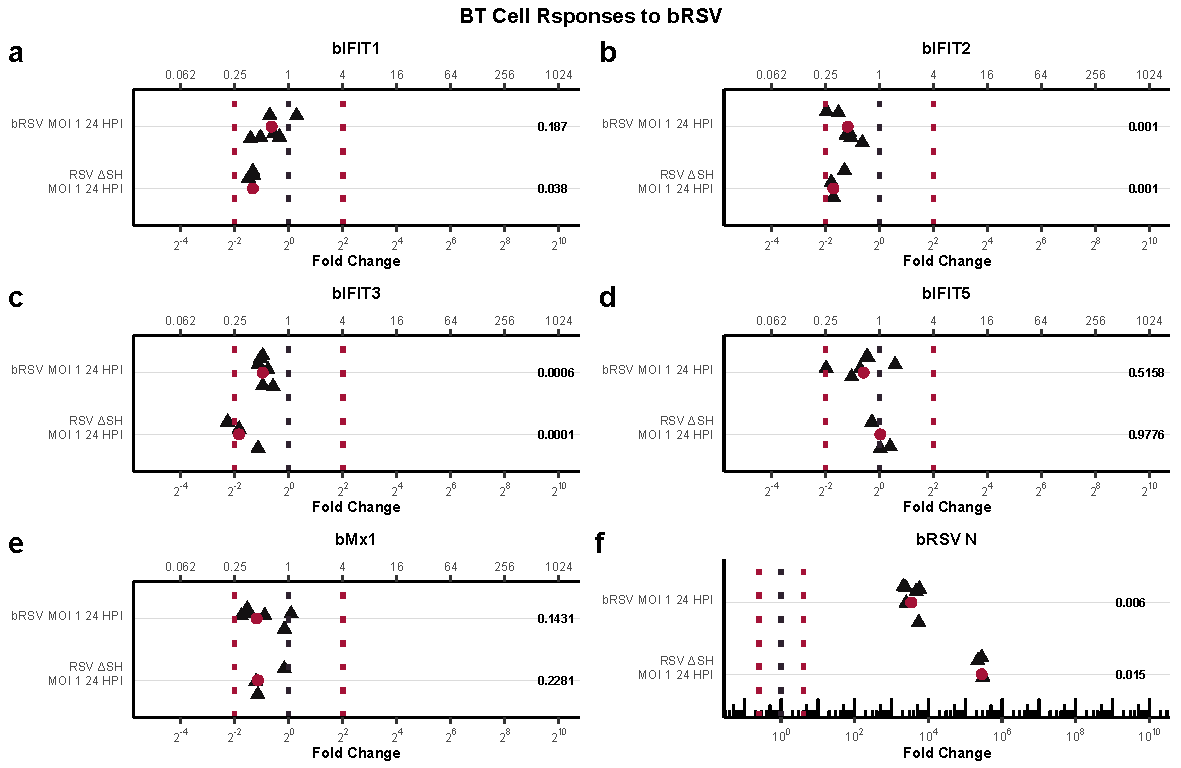
\includegraphics[width=1\linewidth]{07. Chapter 2/Figs/02. Induction/09. bt_brsv.pdf}
    \caption[BT \textit{bIFIT} Response to WT and \(\Delta\)SH bRSV Infection.]{\textbf{BT \textit{bIFIT} Response to WT and \(\Delta\)SH bRSV Infection.} (a) \textit{bIFIT1}, (b) \textit{bIFIT2}, (c) \textit{bIFIT3}, (d) \textit{bIFIT5}, (e) \textit{bMx1}, and (f) \textit{bRSV N} gene expression levels were assessed using quantitative real-time PCR (qPCR) in BT cell line following infection with WT or \(\Delta\)SH bRSV at MOI 1 for 24 hours post-infection. Relative expression values are normalized to standardized mock-treated samples. Median values are represented by red circles. The black dotted line represents mock expression levels, while the red dotted lines indicate biologically significant induction thresholds. Numeric values indicate the p-values compared to mock-treated samples.}
    \label{fig:BT responses to bRSV}
\end{figure}

bt dsh and wt brsv

Infections with wt bRSV and dSH bRSV at the same MOI and HPI (1 and 24) cause slight downregulation in all genes tested.

normal unequal - bi1 brsvn

normal euqal - bi2 bi3 bi5 bmx1

\begin{figure}
    \centering
    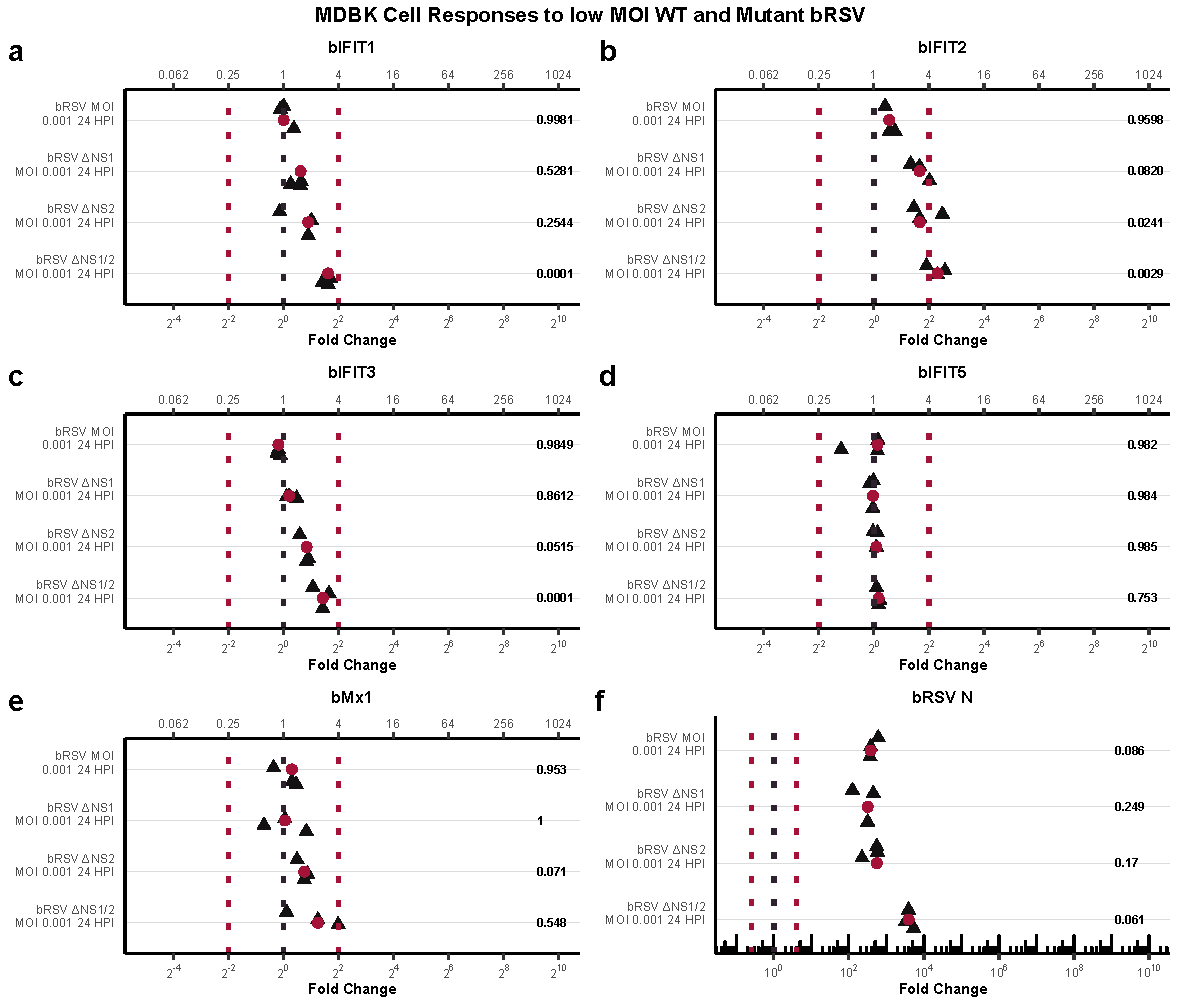
\includegraphics[width=1\linewidth]{07. Chapter 2/Figs/02. Induction/06. mdbk_brsv_low_moi.pdf}
    \caption[MDBK \textit{bIFIT} Response to Low MOI bRSV Infections.]{\textbf{MDBK \textit{bIFIT} Response to Low MOI bRSV Infections.} (a) \textit{bIFIT1}, (b) \textit{bIFIT2}, (c) \textit{bIFIT3}, (d) \textit{bIFIT5}, (e) \textit{bMx1}, and (f) \textit{bRSV N} gene expression levels were assessed using quantitative real-time PCR (qPCR) in MDBK cell line following infection with WT or \(\Delta\)NS1, \(\Delta\)NS2, and \(\Delta\)NS1/2 bRSV at MOIs of 0.001 for 24 hours post-infection. Relative expression values are normalized to standardized mock-treated samples. Median values are represented by red circles. The black dotted line represents mock expression levels, while the red dotted lines indicate biologically significant induction thresholds. Numeric values indicate the p-values compared to mock-treated samples.}
    \label{fig:MDBK responses to low MOI mutant bRSV}
\end{figure}

low moi dnss mdbk

Very low MOI (0.001) wt bRSV along with MOI 1 dSH and very low MOI dNS1, dSN2 and dNS1/2 bRSV do not up or downregulate any genes tested in a biologically significant way.

normal unequal - bi5 bmx1 brsvn

normal euqal - bi1 bi2 bi3 

\subsection{Bovine \textit{IFITs} Responses to hRSV} \label{subsec:Bovine IFITs Responses to hRSV}

Intro into hrsv infections


\begin{figure}
    \centering
    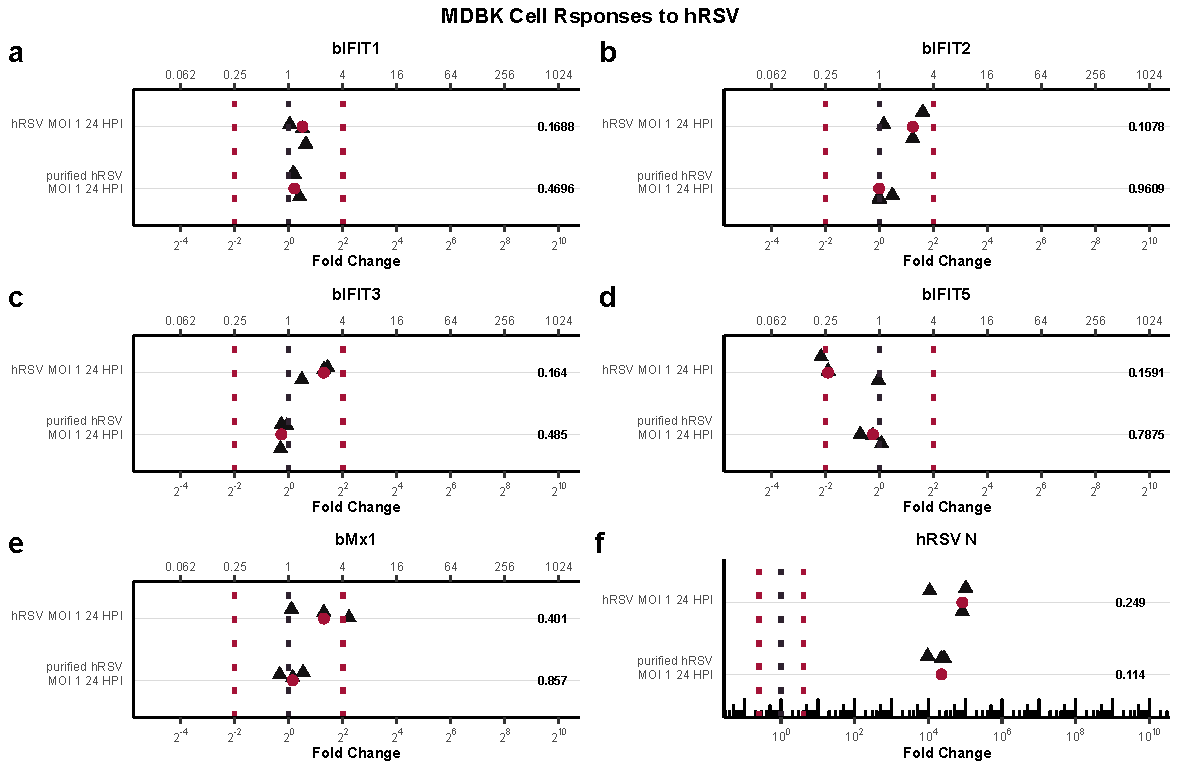
\includegraphics[width=1\linewidth]{07. Chapter 2/Figs/02. Induction/07. mdbk_hrsv.pdf}
    \caption[MDBK \textit{bIFIT} Response to Crude-Extracted and Ultra-Purified hRSV Infection.]{\textbf{MDBK \textit{bIFIT} Response to Crude-Extracted and Ultra-Purified hRSV Infection.} (a) \textit{bIFIT1}, (b) \textit{bIFIT2}, (c) \textit{bIFIT3}, (d) \textit{bIFIT5}, (e) \textit{bMx1}, and (f) \textit{hRSV N} gene expression levels were assessed using quantitative real-time PCR (qPCR) in MDBK cell line following infection with crude-extraccted and ultra-purified hRSV at MOI 1 for 24 hours post-infection. Relative expression values are normalized to standardized mock-treated samples. Median values are represented by red circles. The black dotted line represents mock expression levels, while the red dotted lines indicate biologically significant induction thresholds. Numeric values indicate the p-values compared to mock-treated samples.}
    \label{fig:bIFIT responses to hRSV infection in MDBK}
\end{figure}

mdbk hrsv

Data show that ultracentrifugation purified hRSV causes no response in terms of bIFIT induction. Infection with normally purified virus does not cause induction either but hints at downregulation actually.

normal unequal - bi5 bmx1 brsvn

normal euqal - bi1 bi2 bi3 


\begin{figure}
    \centering
    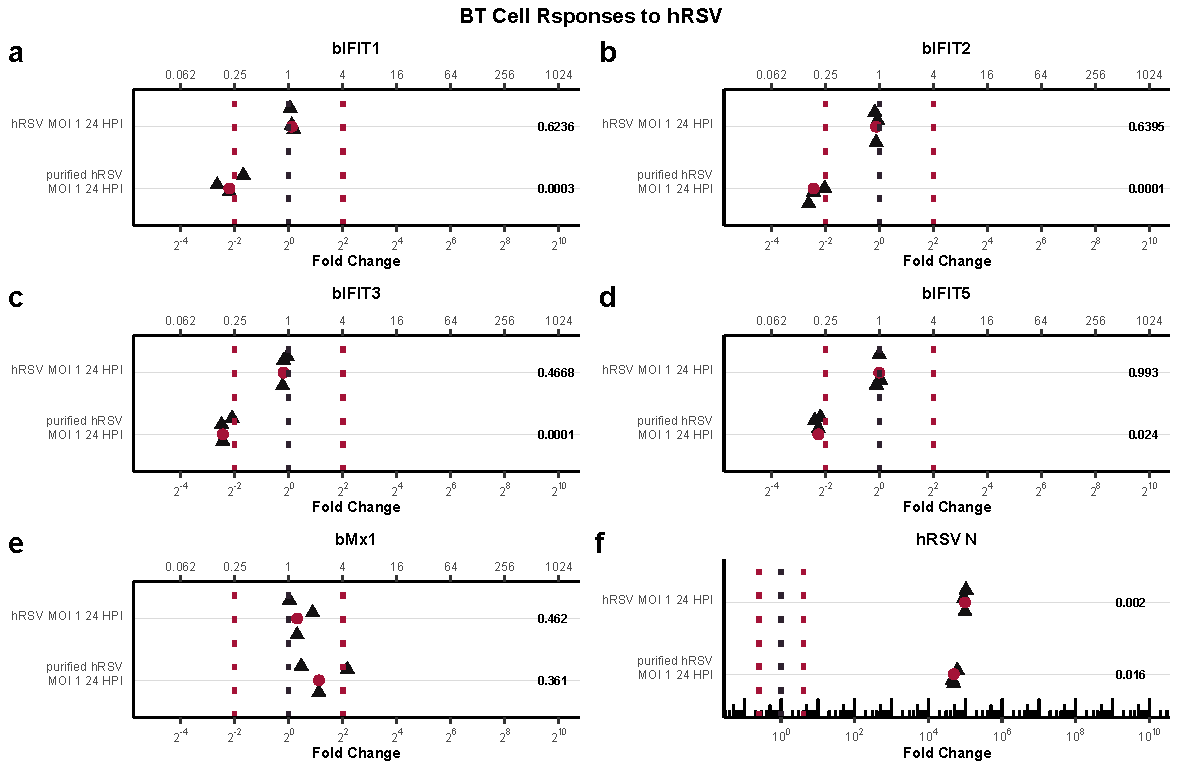
\includegraphics[width=1\linewidth]{07. Chapter 2/Figs/02. Induction/10. bt_hrsv.pdf}
    \caption[BT \textit{bIFIT} Response to Crude-Extracted and Ultra-Purified hRSV Infection.]{\textbf{BT \textit{bIFIT} Response to Crude-Extracted and Ultra-Purified hRSV Infection.} (a) \textit{bIFIT1}, (b) \textit{bIFIT2}, (c) \textit{bIFIT3}, (d) \textit{bIFIT5}, (e) \textit{bMx1}, and (f) \textit{hRSV N} gene expression levels were assessed using quantitative real-time PCR (qPCR) in BT cell line following infection with crude-extraccted and ultra-purified hRSV at MOI 1 for 24 hours post-infection. Relative expression values are normalized to standardized mock-treated samples. Median values are represented by red circles. The black dotted line represents mock expression levels, while the red dotted lines indicate biologically significant induction thresholds. Numeric values indicate the p-values compared to mock-treated samples.}
    \label{fig:Bt responses to hRSV}
\end{figure}

bt hrsv

Ultracentrifugation purified hRSV causes downregulation in IFITs but not bMx1 (where it causes no change), while infection with normally extracted hRSV cause no change in none of the genes tested. 

normal unequal - bi3 bi5 bmx1 hrsvn

normal euqal - bi1 bi2

